\begin{figure}[!htb]

\centerline{
\begin{tikzpicture}[font=\sffamily\footnotesize]
\begin{axis}[
xbar stacked,
y=0.8cm,
%width=5in,
width=\columnwidth,
%height=120pt,
xmin=0,
xmax=100,
bar width=12pt,  
%xmajorgrids=true,
%ylabel={Categorizations},
symbolic y coords={RB, CR, TO, FLT},
ytick=data,
yticklabels={{(d) RB, (c) CR, (b) TO, (a) FLT}},
every axis y label/.style={at={(ticklabel cs:0.5)},rotate=90,anchor=near ticklabel},
xticklabels={,,},
axis x line*=none,
x axis line style={opacity=0},
axis y line*=right
]
\addplot [fill=red!40] plot coordinates {(73.08,RB) (52.88,CR) (88.46,TO) (37.0,FLT)};
\addplot [fill=gray!40] plot coordinates {(20.19,RB) (34.62,CR) (11.54,TO) (63.0,FLT)};
\addplot [fill=pink!40] plot coordinates {(6.73,RB) (7.69,CR) (0,TO) (0,FLT)};
\addplot [fill=brown!40] plot coordinates {(0,RB) (4.81,CR) (0,TO) (0,FLT)};

\coordinate (rb0) at (36.54, -0.5);
\coordinate (rb1) at (83.175, -0.5);
\coordinate (rb2p) at (96.635, -0.5);
\coordinate (cr0) at (26.44, 99.5);
\coordinate (cr1) at (70.19, 99.5);
\coordinate (cr2) at (91.345, 99.5);
\coordinate (cr3p) at (97.595, 99.5);
\coordinate (toNo) at (44.23, 199.5);
\coordinate (toYes) at (94.23, 199.5);
\coordinate (fltNo) at (18.5, 299.5);
\coordinate (fltYes) at (68.5, 299.5);
\end{axis}

\node at (rb0) {0 (73\%)};
\node at (rb1) {1 (20\%)};
\node at (rb2p) {2+};
\node at (cr0) {0 (53\%)};
\node at (cr1) {1 (35\%)};
\node at (cr2) {2 (8\%)};
\node at (cr3p) {3+};
\node at (toNo) {No (88\%)};
\node at (toYes) {Yes (12\%)};
\node at (fltNo) {No (37\%)};
\node at (fltYes) {Yes (63\%)};

\end{tikzpicture}
%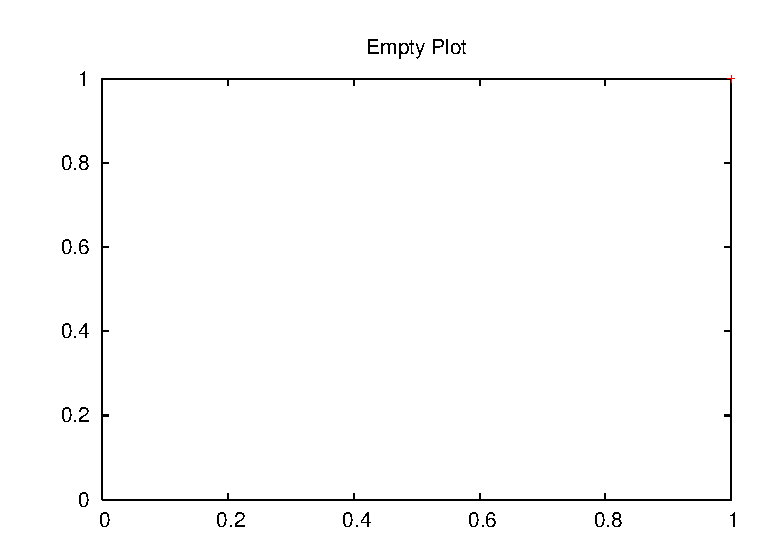
\includegraphics[width=1.8in]{F/empty.eps}
}
\vminten
\mycaption{bars}{Statistical overview of DC bugs}{(a) the percentage of bugs that
require faults; (b) the percentage of bugs that require timeouts; (c) the
percentage of bugs that require the different number of crashes; (d) the
percentages of bugs that require the different number of reboots.}
% \vten

\end{figure}


%
\if 0
nodes (TSN), 
protocols (TSP), 
background (BR), 
triggering messages (TSM), 
local-message race (LM), 
timeout (TO),
crashes (CR),
reboots (RB),
errorMessage (EM),
reported (REP),  
implication (IMP),
control/data plane (CDP), 
\fi
